\documentclass[1p]{elsarticle_modified}
%\bibliographystyle{elsarticle-num}

%\usepackage[colorlinks]{hyperref}
%\usepackage{abbrmath_seonhwa} %\Abb, \Ascr, \Acal ,\Abf, \Afrak
\usepackage{amsfonts}
\usepackage{amssymb}
\usepackage{amsmath}
\usepackage{amsthm}
\usepackage{scalefnt}
\usepackage{amsbsy}
\usepackage{kotex}
\usepackage{caption}
\usepackage{subfig}
\usepackage{color}
\usepackage{graphicx}
\usepackage{xcolor} %% white, black, red, green, blue, cyan, magenta, yellow
\usepackage{float}
\usepackage{setspace}
\usepackage{hyperref}

\usepackage{tikz}
\usetikzlibrary{arrows}

\usepackage{multirow}
\usepackage{array} % fixed length table
\usepackage{hhline}

%%%%%%%%%%%%%%%%%%%%%
\makeatletter
\renewcommand*\env@matrix[1][\arraystretch]{%
	\edef\arraystretch{#1}%
	\hskip -\arraycolsep
	\let\@ifnextchar\new@ifnextchar
	\array{*\c@MaxMatrixCols c}}
\makeatother %https://tex.stackexchange.com/questions/14071/how-can-i-increase-the-line-spacing-in-a-matrix
%%%%%%%%%%%%%%%

\usepackage[normalem]{ulem}

\newcommand{\msout}[1]{\ifmmode\text{\sout{\ensuremath{#1}}}\else\sout{#1}\fi}
%SOURCE: \msout is \stkout macro in https://tex.stackexchange.com/questions/20609/strikeout-in-math-mode

\newcommand{\cancel}[1]{
	\ifmmode
	{\color{red}\msout{#1}}
	\else
	{\color{red}\sout{#1}}
	\fi
}

\newcommand{\add}[1]{
	{\color{blue}\uwave{#1}}
}

\newcommand{\replace}[2]{
	\ifmmode
	{\color{red}\msout{#1}}{\color{blue}\uwave{#2}}
	\else
	{\color{red}\sout{#1}}{\color{blue}\uwave{#2}}
	\fi
}

\newcommand{\Sol}{\mathcal{S}} %segment
\newcommand{\D}{D} %diagram
\newcommand{\A}{\mathcal{A}} %arc


%%%%%%%%%%%%%%%%%%%%%%%%%%%%%5 test

\def\sl{\operatorname{\textup{SL}}(2,\Cbb)}
\def\psl{\operatorname{\textup{PSL}}(2,\Cbb)}
\def\quan{\mkern 1mu \triangleright \mkern 1mu}

\theoremstyle{definition}
\newtheorem{thm}{Theorem}[section]
\newtheorem{prop}[thm]{Proposition}
\newtheorem{lem}[thm]{Lemma}
\newtheorem{ques}[thm]{Question}
\newtheorem{cor}[thm]{Corollary}
\newtheorem{defn}[thm]{Definition}
\newtheorem{exam}[thm]{Example}
\newtheorem{rmk}[thm]{Remark}
\newtheorem{alg}[thm]{Algorithm}

\newcommand{\I}{\sqrt{-1}}
\begin{document}

%\begin{frontmatter}
%
%\title{Boundary parabolic representations of knots up to 8 crossings}
%
%%% Group authors per affiliation:
%\author{Yunhi Cho} 
%\address{Department of Mathematics, University of Seoul, Seoul, Korea}
%\ead{yhcho@uos.ac.kr}
%
%
%\author{Seonhwa Kim} %\fnref{s_kim}}
%\address{Center for Geometry and Physics, Institute for Basic Science, Pohang, 37673, Korea}
%\ead{ryeona17@ibs.re.kr}
%
%\author{Hyuk Kim}
%\address{Department of Mathematical Sciences, Seoul National University, Seoul 08826, Korea}
%\ead{hyukkim@snu.ac.kr}
%
%\author{Seokbeom Yoon}
%\address{Department of Mathematical Sciences, Seoul National University, Seoul, 08826,  Korea}
%\ead{sbyoon15@snu.ac.kr}
%
%\begin{abstract}
%We find all boundary parabolic representation of knots up to 8 crossings.
%
%\end{abstract}
%\begin{keyword}
%    \MSC[2010] 57M25 
%\end{keyword}
%
%\end{frontmatter}

%\linenumbers
%\tableofcontents
%
\newcommand\colored[1]{\textcolor{white}{\rule[-0.35ex]{0.8em}{1.4ex}}\kern-0.8em\color{red} #1}%
%\newcommand\colored[1]{\textcolor{white}{ #1}\kern-2.17ex	\textcolor{white}{ #1}\kern-1.81ex	\textcolor{white}{ #1}\kern-2.15ex\color{red}#1	}

{\Large $\underline{12n_{0417}~(K12n_{0417})}$}

\setlength{\tabcolsep}{10pt}
\renewcommand{\arraystretch}{1.6}
\vspace{1cm}\begin{tabular}{m{100pt}>{\centering\arraybackslash}m{274pt}}
\multirow{5}{120pt}{
	\centering
	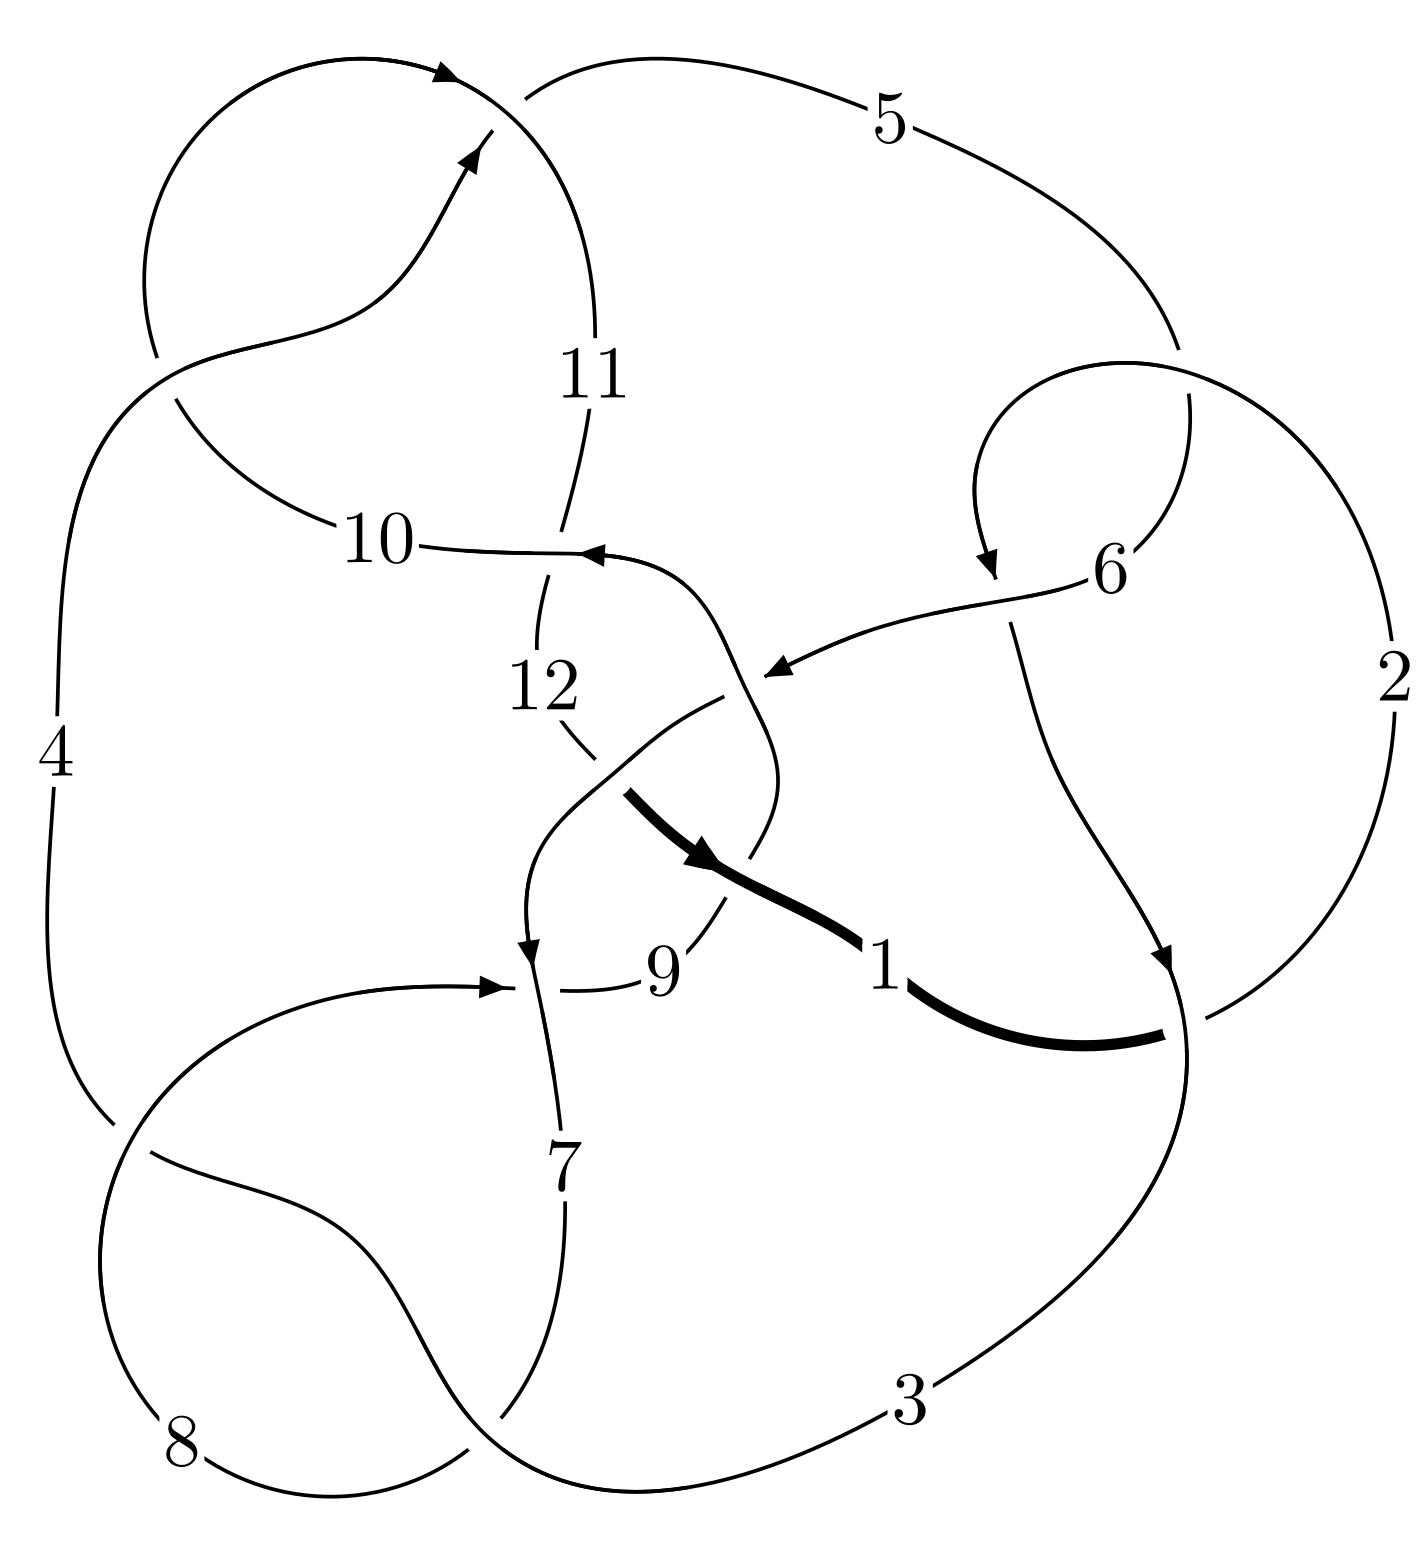
\includegraphics[width=112pt]{../../../GIT/diagram.site/Diagrams/png/2506_12n_0417.png}\\
\ \ \ A knot diagram\footnotemark}&
\allowdisplaybreaks
\textbf{Linearized knot diagam} \\
\cline{2-2}
 &
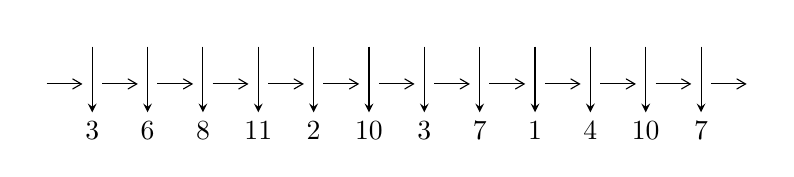
\begin{tikzpicture}[x=20pt, y=17pt]
	% nodes
	\node (C0) at (0, 0) {};
	\node (C1) at (1, 0) {};
	\node (C1U) at (1, +1) {};
	\node (C1D) at (1, -1) {3};

	\node (C2) at (2, 0) {};
	\node (C2U) at (2, +1) {};
	\node (C2D) at (2, -1) {6};

	\node (C3) at (3, 0) {};
	\node (C3U) at (3, +1) {};
	\node (C3D) at (3, -1) {8};

	\node (C4) at (4, 0) {};
	\node (C4U) at (4, +1) {};
	\node (C4D) at (4, -1) {11};

	\node (C5) at (5, 0) {};
	\node (C5U) at (5, +1) {};
	\node (C5D) at (5, -1) {2};

	\node (C6) at (6, 0) {};
	\node (C6U) at (6, +1) {};
	\node (C6D) at (6, -1) {10};

	\node (C7) at (7, 0) {};
	\node (C7U) at (7, +1) {};
	\node (C7D) at (7, -1) {3};

	\node (C8) at (8, 0) {};
	\node (C8U) at (8, +1) {};
	\node (C8D) at (8, -1) {7};

	\node (C9) at (9, 0) {};
	\node (C9U) at (9, +1) {};
	\node (C9D) at (9, -1) {1};

	\node (C10) at (10, 0) {};
	\node (C10U) at (10, +1) {};
	\node (C10D) at (10, -1) {4};

	\node (C11) at (11, 0) {};
	\node (C11U) at (11, +1) {};
	\node (C11D) at (11, -1) {10};

	\node (C12) at (12, 0) {};
	\node (C12U) at (12, +1) {};
	\node (C12D) at (12, -1) {7};
	\node (C13) at (13, 0) {};

	% arrows
	\draw[->,>={angle 60}]
	(C0) edge (C1) (C1) edge (C2) (C2) edge (C3) (C3) edge (C4) (C4) edge (C5) (C5) edge (C6) (C6) edge (C7) (C7) edge (C8) (C8) edge (C9) (C9) edge (C10) (C10) edge (C11) (C11) edge (C12) (C12) edge (C13) ;	\draw[->,>=stealth]
	(C1U) edge (C1D) (C2U) edge (C2D) (C3U) edge (C3D) (C4U) edge (C4D) (C5U) edge (C5D) (C6U) edge (C6D) (C7U) edge (C7D) (C8U) edge (C8D) (C9U) edge (C9D) (C10U) edge (C10D) (C11U) edge (C11D) (C12U) edge (C12D) ;
	\end{tikzpicture} \\
\hhline{~~} \\& 
\textbf{Solving Sequence} \\ \cline{2-2} 
 &
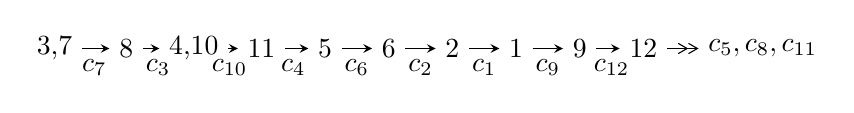
\begin{tikzpicture}[x=23pt, y=7pt]
	% node
	\node (A0) at (-1/8, 0) {3,7};
	\node (A1) at (1, 0) {8};
	\node (A2) at (33/16, 0) {4,10};
	\node (A3) at (25/8, 0) {11};
	\node (A4) at (33/8, 0) {5};
	\node (A5) at (41/8, 0) {6};
	\node (A6) at (49/8, 0) {2};
	\node (A7) at (57/8, 0) {1};
	\node (A8) at (65/8, 0) {9};
	\node (A9) at (73/8, 0) {12};
	\node (C1) at (1/2, -1) {$c_{7}$};
	\node (C2) at (3/2, -1) {$c_{3}$};
	\node (C3) at (21/8, -1) {$c_{10}$};
	\node (C4) at (29/8, -1) {$c_{4}$};
	\node (C5) at (37/8, -1) {$c_{6}$};
	\node (C6) at (45/8, -1) {$c_{2}$};
	\node (C7) at (53/8, -1) {$c_{1}$};
	\node (C8) at (61/8, -1) {$c_{9}$};
	\node (C9) at (69/8, -1) {$c_{12}$};
	\node (A10) at (11, 0) {$c_{5},c_{8},c_{11}$};

	% edge
	\draw[->,>=stealth]	
	(A0) edge (A1) (A1) edge (A2) (A2) edge (A3) (A3) edge (A4) (A4) edge (A5) (A5) edge (A6) (A6) edge (A7) (A7) edge (A8) (A8) edge (A9) ;
	\draw[->>,>={angle 60}]	
	(A9) edge (A10);
\end{tikzpicture} \\ 

\end{tabular} \\

\footnotetext{
The image of knot diagram is generated by the software ``\textbf{Draw programme}" developed by Andrew Bartholomew(\url{http://www.layer8.co.uk/maths/draw/index.htm\#Running-draw}), where we modified some parts for our purpose(\url{https://github.com/CATsTAILs/LinksPainter}).
}\phantom \\ \newline 
\centering \textbf{Ideals for irreducible components\footnotemark of $X_{\text{par}}$} 
 
\begin{align*}
I^u_{1}&=\langle 
536 u^{11}-335 u^{10}+\cdots+239 b+523,\;-947 u^{11}+562 u^{10}+\cdots+239 a-1324,\\
\phantom{I^u_{1}}&\phantom{= \langle  }u^{12}-4 u^{10}+13 u^8-2 u^7-24 u^6-3 u^5+18 u^4+3 u^3-7 u^2- u+1\rangle \\
I^u_{2}&=\langle 
u^6-3 u^4+3 u^2+b+u-1,\;- u^6+u^5+4 u^4-3 u^3-5 u^2+a+2 u+3,\;u^7-4 u^5+6 u^3+u^2-4 u-1\rangle \\
I^u_{3}&=\langle 
68215362482207 u^{19}+127486835274380 u^{18}+\cdots+1057281252711 b+705066157444833,\\
\phantom{I^u_{3}}&\phantom{= \langle  }298873575023330 u^{19}+558685165549478 u^{18}+\cdots+3171843758133 a+3089653339595532,\\
\phantom{I^u_{3}}&\phantom{= \langle  }u^{20}+u^{19}+\cdots+18 u-9\rangle \\
I^u_{4}&=\langle 
u^6-3 u^4- u^3+2 u^2+b-2,\;- u^7+3 u^5+u^4-2 u^3+u^2+a+2 u-2,\;u^8-4 u^6- u^5+5 u^4+u^3-4 u^2+1\rangle \\
\\
\end{align*}
\raggedright * 4 irreducible components of $\dim_{\mathbb{C}}=0$, with total 47 representations.\\
\footnotetext{All coefficients of polynomials are rational numbers. But the coefficients are sometimes approximated in decimal forms when there is not enough margin.}
\newpage
\renewcommand{\arraystretch}{1}
\centering \section*{I. $I^u_{1}= \langle 536 u^{11}-335 u^{10}+\cdots+239 b+523,\;-947 u^{11}+562 u^{10}+\cdots+239 a-1324,\;u^{12}-4 u^{10}+\cdots- u+1 \rangle$}
\flushleft \textbf{(i) Arc colorings}\\
\begin{tabular}{m{7pt} m{180pt} m{7pt} m{180pt} }
\flushright $a_{3}=$&$\begin{pmatrix}0\\u\end{pmatrix}$ \\
\flushright $a_{7}=$&$\begin{pmatrix}1\\0\end{pmatrix}$ \\
\flushright $a_{8}=$&$\begin{pmatrix}1\\u^2\end{pmatrix}$ \\
\flushright $a_{4}=$&$\begin{pmatrix}- u\\- u^3+u\end{pmatrix}$ \\
\flushright $a_{10}=$&$\begin{pmatrix}3.96234 u^{11}-2.35146 u^{10}+\cdots-11.8033 u+5.53975\\-2.24268 u^{11}+1.40167 u^{10}+\cdots+5.48954 u-2.18828\end{pmatrix}$ \\
\flushright $a_{11}=$&$\begin{pmatrix}3.96234 u^{11}-2.35146 u^{10}+\cdots-11.8033 u+5.53975\\-2.24268 u^{11}+1.40167 u^{10}+\cdots+5.48954 u-2.18828\end{pmatrix}$ \\
\flushright $a_{5}=$&$\begin{pmatrix}2.35146 u^{11}-1.71967 u^{10}+\cdots-10.5021 u+3.96234\\-1.40167 u^{11}+1.25105 u^{10}+\cdots+5.43096 u-2.24268\end{pmatrix}$ \\
\flushright $a_{6}=$&$\begin{pmatrix}0.589958 u^{11}-0.493724 u^{10}+\cdots+1.58577 u+0.543933\\2.71130 u^{11}-1.69456 u^{10}+\cdots-8.15900 u+3.13808\end{pmatrix}$ \\
\flushright $a_{2}=$&$\begin{pmatrix}3.23431 u^{11}-2.14644 u^{10}+\cdots-7.33473 u+3.97490\\0.974895 u^{11}-0.234310 u^{10}+\cdots-3.53556 u+1.35983\end{pmatrix}$ \\
\flushright $a_{1}=$&$\begin{pmatrix}3.23431 u^{11}-2.14644 u^{10}+\cdots-7.33473 u+3.97490\\-0.991632 u^{11}+0.744770 u^{10}+\cdots+1.84519 u-0.786611\end{pmatrix}$ \\
\flushright $a_{9}=$&$\begin{pmatrix}- u^2+1\\u^2\end{pmatrix}$ \\
\flushright $a_{12}=$&$\begin{pmatrix}2.24268 u^{11}-1.40167 u^{10}+\cdots-5.48954 u+3.18828\\-0.991632 u^{11}+0.744770 u^{10}+\cdots+1.84519 u-0.786611\end{pmatrix}$\\&\end{tabular}
\flushleft \textbf{(ii) Obstruction class $= -1$}\\~\\
\flushleft \textbf{(iii) Cusp Shapes $= -\frac{1675}{239} u^{11}+\frac{1734}{239} u^{10}+\frac{5437}{239} u^9-\frac{5818}{239} u^8-\frac{17601}{239} u^7+\frac{22148}{239} u^6+\frac{23370}{239} u^5-\frac{22069}{239} u^4-\frac{17044}{239} u^3+\frac{13395}{239} u^2+\frac{5056}{239} u-\frac{6743}{239}$}\\~\\
\newpage\renewcommand{\arraystretch}{1}
\flushleft \textbf{(iv) u-Polynomials at the component}\newline \\
\begin{tabular}{m{50pt}|m{274pt}}
Crossings & \hspace{64pt}u-Polynomials at each crossing \\
\hline $$\begin{aligned}c_{1}\end{aligned}$$&$\begin{aligned}
&u^{12}+6 u^{11}+\cdots+848 u+64
\end{aligned}$\\
\hline $$\begin{aligned}c_{2},c_{5}\end{aligned}$$&$\begin{aligned}
&u^{12}+8 u^{11}+\cdots+52 u+8
\end{aligned}$\\
\hline $$\begin{aligned}c_{3},c_{4},c_{7}\\c_{10}\end{aligned}$$&$\begin{aligned}
&u^{12}-4 u^{10}+13 u^8+2 u^7-24 u^6+3 u^5+18 u^4-3 u^3-7 u^2+u+1
\end{aligned}$\\
\hline $$\begin{aligned}c_{6},c_{9}\end{aligned}$$&$\begin{aligned}
&u^{12}+u^{11}+\cdots+8 u+1
\end{aligned}$\\
\hline $$\begin{aligned}c_{8},c_{11}\end{aligned}$$&$\begin{aligned}
&u^{12}+8 u^{11}+\cdots+15 u+1
\end{aligned}$\\
\hline $$\begin{aligned}c_{12}\end{aligned}$$&$\begin{aligned}
&u^{12}+10 u^{11}+\cdots-196 u-20
\end{aligned}$\\
\hline
\end{tabular}\\~\\
\newpage\renewcommand{\arraystretch}{1}
\flushleft \textbf{(v) Riley Polynomials at the component}\newline \\
\begin{tabular}{m{50pt}|m{274pt}}
Crossings & \hspace{64pt}Riley Polynomials at each crossing \\
\hline $$\begin{aligned}c_{1}\end{aligned}$$&$\begin{aligned}
&y^{12}+18 y^{11}+\cdots-419072 y+4096
\end{aligned}$\\
\hline $$\begin{aligned}c_{2},c_{5}\end{aligned}$$&$\begin{aligned}
&y^{12}-6 y^{11}+\cdots-848 y+64
\end{aligned}$\\
\hline $$\begin{aligned}c_{3},c_{4},c_{7}\\c_{10}\end{aligned}$$&$\begin{aligned}
&y^{12}-8 y^{11}+\cdots-15 y+1
\end{aligned}$\\
\hline $$\begin{aligned}c_{6},c_{9}\end{aligned}$$&$\begin{aligned}
&y^{12}+11 y^{11}+\cdots-16 y+1
\end{aligned}$\\
\hline $$\begin{aligned}c_{8},c_{11}\end{aligned}$$&$\begin{aligned}
&y^{12}+20 y^{11}+\cdots-43 y+1
\end{aligned}$\\
\hline $$\begin{aligned}c_{12}\end{aligned}$$&$\begin{aligned}
&y^{12}-40 y^{11}+\cdots-4496 y+400
\end{aligned}$\\
\hline
\end{tabular}\\~\\
\newpage\flushleft \textbf{(vi) Complex Volumes and Cusp Shapes}
$$\begin{array}{c|c|c}  
\text{Solutions to }I^u_{1}& \I (\text{vol} + \sqrt{-1}CS) & \text{Cusp shape}\\
 \hline 
\begin{aligned}
u &= -0.790520 + 0.392533 I \\
a &= -0.333077 - 0.431942 I \\
b &= \phantom{-}0.908183 + 0.435278 I\end{aligned}
 & -3.78101 + 0.45111 I & -18.5516 - 2.4488 I \\ \hline\begin{aligned}
u &= -0.790520 - 0.392533 I \\
a &= -0.333077 + 0.431942 I \\
b &= \phantom{-}0.908183 - 0.435278 I\end{aligned}
 & -3.78101 - 0.45111 I & -18.5516 + 2.4488 I \\ \hline\begin{aligned}
u &= -0.736086 + 0.101541 I \\
a &= \phantom{-}1.55509 + 1.56812 I \\
b &= \phantom{-}0.505873 - 0.967109 I\end{aligned}
 & -0.21900 + 4.19269 I & -13.9112 - 5.3421 I \\ \hline\begin{aligned}
u &= -0.736086 - 0.101541 I \\
a &= \phantom{-}1.55509 - 1.56812 I \\
b &= \phantom{-}0.505873 + 0.967109 I\end{aligned}
 & -0.21900 - 4.19269 I & -13.9112 + 5.3421 I \\ \hline\begin{aligned}
u &= \phantom{-}0.653112 + 0.249393 I \\
a &= \phantom{-}1.71916 - 0.21403 I \\
b &= -0.023047 + 0.696086 I\end{aligned}
 & -0.134851 + 0.667722 I & -12.59936 + 0.82514 I \\ \hline\begin{aligned}
u &= \phantom{-}0.653112 - 0.249393 I \\
a &= \phantom{-}1.71916 + 0.21403 I \\
b &= -0.023047 - 0.696086 I\end{aligned}
 & -0.134851 - 0.667722 I & -12.59936 - 0.82514 I \\ \hline\begin{aligned}
u &= \phantom{-}1.54915\phantom{ +0.000000I} \\
a &= -0.373370\phantom{ +0.000000I} \\
b &= \phantom{-}0.477327\phantom{ +0.000000I}\end{aligned}
 & -15.2923\phantom{ +0.000000I} & -6.68440\phantom{ +0.000000I} \\ \hline\begin{aligned}
u &= \phantom{-}0.403757\phantom{ +0.000000I} \\
a &= \phantom{-}0.897573\phantom{ +0.000000I} \\
b &= \phantom{-}0.248749\phantom{ +0.000000I}\end{aligned}
 & -0.603932\phantom{ +0.000000I} & -16.3720\phantom{ +0.000000I} \\ \hline\begin{aligned}
u &= -1.36080 + 0.93328 I \\
a &= -0.627613 - 0.831271 I \\
b &= -1.09936 + 1.61015 I\end{aligned}
 & \phantom{-}5.78267 + 12.88920 I & -12.7241 - 6.3496 I \\ \hline\begin{aligned}
u &= -1.36080 - 0.93328 I \\
a &= -0.627613 + 0.831271 I \\
b &= -1.09936 - 1.61015 I\end{aligned}
 & \phantom{-}5.78267 - 12.88920 I & -12.7241 + 6.3496 I\\
 \hline 
 \end{array}$$\newpage$$\begin{array}{c|c|c}  
\text{Solutions to }I^u_{1}& \I (\text{vol} + \sqrt{-1}CS) & \text{Cusp shape}\\
 \hline 
\begin{aligned}
u &= \phantom{-}1.25783 + 1.10048 I \\
a &= -0.575658 + 0.547864 I \\
b &= -0.15469 - 1.93823 I\end{aligned}
 & \phantom{-}7.12277 - 3.83904 I & -10.68570 + 2.08253 I \\ \hline\begin{aligned}
u &= \phantom{-}1.25783 - 1.10048 I \\
a &= -0.575658 - 0.547864 I \\
b &= -0.15469 + 1.93823 I\end{aligned}
 & \phantom{-}7.12277 + 3.83904 I & -10.68570 - 2.08253 I\\
 \hline 
 \end{array}$$\newpage\newpage\renewcommand{\arraystretch}{1}
\centering \section*{II. $I^u_{2}= \langle u^6-3 u^4+3 u^2+b+u-1,\;- u^6+u^5+4 u^4-3 u^3-5 u^2+a+2 u+3,\;u^7-4 u^5+6 u^3+u^2-4 u-1 \rangle$}
\flushleft \textbf{(i) Arc colorings}\\
\begin{tabular}{m{7pt} m{180pt} m{7pt} m{180pt} }
\flushright $a_{3}=$&$\begin{pmatrix}0\\u\end{pmatrix}$ \\
\flushright $a_{7}=$&$\begin{pmatrix}1\\0\end{pmatrix}$ \\
\flushright $a_{8}=$&$\begin{pmatrix}1\\u^2\end{pmatrix}$ \\
\flushright $a_{4}=$&$\begin{pmatrix}- u\\- u^3+u\end{pmatrix}$ \\
\flushright $a_{10}=$&$\begin{pmatrix}u^6- u^5-4 u^4+3 u^3+5 u^2-2 u-3\\- u^6+3 u^4-3 u^2- u+1\end{pmatrix}$ \\
\flushright $a_{11}=$&$\begin{pmatrix}u^6- u^5-4 u^4+3 u^3+6 u^2-2 u-3\\- u^6+4 u^4-4 u^2- u+1\end{pmatrix}$ \\
\flushright $a_{5}=$&$\begin{pmatrix}- u^6+3 u^4-3 u^2+1\\u^3-2 u-1\end{pmatrix}$ \\
\flushright $a_{6}=$&$\begin{pmatrix}- u^6+4 u^4- u^3-6 u^2+u+4\\- u^5- u^4+3 u^3+2 u^2-3 u-2\end{pmatrix}$ \\
\flushright $a_{2}=$&$\begin{pmatrix}u^6-4 u^4+5 u^2+u-3\\u+1\end{pmatrix}$ \\
\flushright $a_{1}=$&$\begin{pmatrix}u^6-4 u^4+5 u^2+u-3\\u^4- u^2+1\end{pmatrix}$ \\
\flushright $a_{9}=$&$\begin{pmatrix}- u^2+1\\u^2\end{pmatrix}$ \\
\flushright $a_{12}=$&$\begin{pmatrix}u^6-3 u^4+4 u^2+u-2\\u^4- u^2+1\end{pmatrix}$\\&\end{tabular}
\flushleft \textbf{(ii) Obstruction class $= 1$}\\~\\
\flushleft \textbf{(iii) Cusp Shapes $= -5 u^6+4 u^5+13 u^4-10 u^3-11 u^2+4 u-8$}\\~\\
\newpage\renewcommand{\arraystretch}{1}
\flushleft \textbf{(iv) u-Polynomials at the component}\newline \\
\begin{tabular}{m{50pt}|m{274pt}}
Crossings & \hspace{64pt}u-Polynomials at each crossing \\
\hline $$\begin{aligned}c_{1}\end{aligned}$$&$\begin{aligned}
&u^7-7 u^6+21 u^5-37 u^4+37 u^3-24 u^2+9 u-1
\end{aligned}$\\
\hline $$\begin{aligned}c_{2}\end{aligned}$$&$\begin{aligned}
&u^7+u^6-3 u^5-5 u^4+u^3+4 u^2+u-1
\end{aligned}$\\
\hline $$\begin{aligned}c_{3},c_{10}\end{aligned}$$&$\begin{aligned}
&u^7-4 u^5+6 u^3- u^2-4 u+1
\end{aligned}$\\
\hline $$\begin{aligned}c_{4},c_{7}\end{aligned}$$&$\begin{aligned}
&u^7-4 u^5+6 u^3+u^2-4 u-1
\end{aligned}$\\
\hline $$\begin{aligned}c_{5}\end{aligned}$$&$\begin{aligned}
&u^7- u^6-3 u^5+5 u^4+u^3-4 u^2+u+1
\end{aligned}$\\
\hline $$\begin{aligned}c_{6},c_{9}\end{aligned}$$&$\begin{aligned}
&u^7+u^6+u^4- u^3- u^2- u-1
\end{aligned}$\\
\hline $$\begin{aligned}c_{8},c_{11}\end{aligned}$$&$\begin{aligned}
&u^7+8 u^6+28 u^5+56 u^4+68 u^3+49 u^2+18 u+1
\end{aligned}$\\
\hline $$\begin{aligned}c_{12}\end{aligned}$$&$\begin{aligned}
&u^7+7 u^6+17 u^5+30 u^4+45 u^3+27 u^2+6 u+4
\end{aligned}$\\
\hline
\end{tabular}\\~\\
\newpage\renewcommand{\arraystretch}{1}
\flushleft \textbf{(v) Riley Polynomials at the component}\newline \\
\begin{tabular}{m{50pt}|m{274pt}}
Crossings & \hspace{64pt}Riley Polynomials at each crossing \\
\hline $$\begin{aligned}c_{1}\end{aligned}$$&$\begin{aligned}
&y^7-7 y^6-3 y^5-133 y^4-43 y^3+16 y^2+33 y-1
\end{aligned}$\\
\hline $$\begin{aligned}c_{2},c_{5}\end{aligned}$$&$\begin{aligned}
&y^7-7 y^6+21 y^5-37 y^4+37 y^3-24 y^2+9 y-1
\end{aligned}$\\
\hline $$\begin{aligned}c_{3},c_{4},c_{7}\\c_{10}\end{aligned}$$&$\begin{aligned}
&y^7-8 y^6+28 y^5-56 y^4+68 y^3-49 y^2+18 y-1
\end{aligned}$\\
\hline $$\begin{aligned}c_{6},c_{9}\end{aligned}$$&$\begin{aligned}
&y^7- y^6-4 y^5- y^4+5 y^3+3 y^2- y-1
\end{aligned}$\\
\hline $$\begin{aligned}c_{8},c_{11}\end{aligned}$$&$\begin{aligned}
&y^7-8 y^6+24 y^5-76 y^4+128 y^3-65 y^2+226 y-1
\end{aligned}$\\
\hline $$\begin{aligned}c_{12}\end{aligned}$$&$\begin{aligned}
&y^7-15 y^6-41 y^5+264 y^4+553 y^3-429 y^2-180 y-16
\end{aligned}$\\
\hline
\end{tabular}\\~\\
\newpage\flushleft \textbf{(vi) Complex Volumes and Cusp Shapes}
$$\begin{array}{c|c|c}  
\text{Solutions to }I^u_{2}& \I (\text{vol} + \sqrt{-1}CS) & \text{Cusp shape}\\
 \hline 
\begin{aligned}
u &= -0.970575 + 0.467764 I \\
a &= \phantom{-}0.61390 + 1.62676 I \\
b &= \phantom{-}0.307176 - 1.007690 I\end{aligned}
 & -0.15907 + 5.95632 I & -10.30399 - 9.49474 I \\ \hline\begin{aligned}
u &= -0.970575 - 0.467764 I \\
a &= \phantom{-}0.61390 - 1.62676 I \\
b &= \phantom{-}0.307176 + 1.007690 I\end{aligned}
 & -0.15907 - 5.95632 I & -10.30399 + 9.49474 I \\ \hline\begin{aligned}
u &= \phantom{-}1.28252\phantom{ +0.000000I} \\
a &= -0.853969\phantom{ +0.000000I} \\
b &= -1.55070\phantom{ +0.000000I}\end{aligned}
 & -9.96367\phantom{ +0.000000I} & -15.2580\phantom{ +0.000000I} \\ \hline\begin{aligned}
u &= \phantom{-}1.219310 + 0.473158 I \\
a &= \phantom{-}0.831288 - 0.514652 I \\
b &= -0.187678 + 0.823913 I\end{aligned}
 & -1.96867 - 1.64297 I & -12.60937 + 1.83263 I \\ \hline\begin{aligned}
u &= \phantom{-}1.219310 - 0.473158 I \\
a &= \phantom{-}0.831288 + 0.514652 I \\
b &= -0.187678 - 0.823913 I\end{aligned}
 & -1.96867 + 1.64297 I & -12.60937 - 1.83263 I \\ \hline\begin{aligned}
u &= -1.52200\phantom{ +0.000000I} \\
a &= \phantom{-}0.182606\phantom{ +0.000000I} \\
b &= -0.759603\phantom{ +0.000000I}\end{aligned}
 & -15.6521\phantom{ +0.000000I} & -29.3740\phantom{ +0.000000I} \\ \hline\begin{aligned}
u &= -0.257994\phantom{ +0.000000I} \\
a &= -2.21901\phantom{ +0.000000I} \\
b &= \phantom{-}1.07131\phantom{ +0.000000I}\end{aligned}
 & -3.02746\phantom{ +0.000000I} & -9.54090\phantom{ +0.000000I}\\
 \hline 
 \end{array}$$\newpage\newpage\renewcommand{\arraystretch}{1}
\centering \section*{III. $I^u_{3}= \langle 6.82\times10^{13} u^{19}+1.27\times10^{14} u^{18}+\cdots+1.06\times10^{12} b+7.05\times10^{14},\;2.99\times10^{14} u^{19}+5.59\times10^{14} u^{18}+\cdots+3.17\times10^{12} a+3.09\times10^{15},\;u^{20}+u^{19}+\cdots+18 u-9 \rangle$}
\flushleft \textbf{(i) Arc colorings}\\
\begin{tabular}{m{7pt} m{180pt} m{7pt} m{180pt} }
\flushright $a_{3}=$&$\begin{pmatrix}0\\u\end{pmatrix}$ \\
\flushright $a_{7}=$&$\begin{pmatrix}1\\0\end{pmatrix}$ \\
\flushright $a_{8}=$&$\begin{pmatrix}1\\u^2\end{pmatrix}$ \\
\flushright $a_{4}=$&$\begin{pmatrix}- u\\- u^3+u\end{pmatrix}$ \\
\flushright $a_{10}=$&$\begin{pmatrix}-94.2271 u^{19}-176.139 u^{18}+\cdots+828.728 u-974.087\\-64.5196 u^{19}-120.580 u^{18}+\cdots+565.622 u-666.867\end{pmatrix}$ \\
\flushright $a_{11}=$&$\begin{pmatrix}-27.9506 u^{19}-52.2643 u^{18}+\cdots+246.326 u-288.781\\-80.6876 u^{19}-150.746 u^{18}+\cdots+707.746 u-833.790\end{pmatrix}$ \\
\flushright $a_{5}=$&$\begin{pmatrix}4.98357 u^{19}+9.51307 u^{18}+\cdots-45.9289 u+48.9194\\-99.9143 u^{19}-186.269 u^{18}+\cdots+873.984 u-1037.72\end{pmatrix}$ \\
\flushright $a_{6}=$&$\begin{pmatrix}-68.8452 u^{19}-128.348 u^{18}+\cdots+604.749 u-717.167\\-76.2363 u^{19}-142.302 u^{18}+\cdots+674.421 u-794.311\end{pmatrix}$ \\
\flushright $a_{2}=$&$\begin{pmatrix}69.0216 u^{19}+129.223 u^{18}+\cdots-608.826 u+712.093\\105.226 u^{19}+196.557 u^{18}+\cdots-922.384 u+1090.86\end{pmatrix}$ \\
\flushright $a_{1}=$&$\begin{pmatrix}69.0216 u^{19}+129.223 u^{18}+\cdots-608.826 u+712.093\\52.6964 u^{19}+98.1510 u^{18}+\cdots-459.959 u+549.054\end{pmatrix}$ \\
\flushright $a_{9}=$&$\begin{pmatrix}- u^2+1\\u^2\end{pmatrix}$ \\
\flushright $a_{12}=$&$\begin{pmatrix}121.718 u^{19}+227.374 u^{18}+\cdots-1068.79 u+1261.15\\52.6964 u^{19}+98.1510 u^{18}+\cdots-459.959 u+549.054\end{pmatrix}$\\&\end{tabular}
\flushleft \textbf{(ii) Obstruction class $= -1$}\\~\\
\flushleft \textbf{(iii) Cusp Shapes $= -\frac{128749727823573}{352427084237} u^{19}-\frac{240297448875642}{352427084237} u^{18}+\cdots+\frac{1127484403652596}{352427084237} u-\frac{1338735790487557}{352427084237}$}\\~\\
\newpage\renewcommand{\arraystretch}{1}
\flushleft \textbf{(iv) u-Polynomials at the component}\newline \\
\begin{tabular}{m{50pt}|m{274pt}}
Crossings & \hspace{64pt}u-Polynomials at each crossing \\
\hline $$\begin{aligned}c_{1}\end{aligned}$$&$\begin{aligned}
&(u^{10}+u^9+8 u^8+12 u^7-8 u^6-6 u^5-4 u^4+21 u^3+21 u^2+14 u+1)^2
\end{aligned}$\\
\hline $$\begin{aligned}c_{2},c_{5}\end{aligned}$$&$\begin{aligned}
&(u^{10}-3 u^9+4 u^8-2 u^7+2 u^6-4 u^5- u^3+5 u^2-2 u-1)^2
\end{aligned}$\\
\hline $$\begin{aligned}c_{3},c_{4},c_{7}\\c_{10}\end{aligned}$$&$\begin{aligned}
&u^{20}- u^{19}+\cdots-18 u-9
\end{aligned}$\\
\hline $$\begin{aligned}c_{6},c_{9}\end{aligned}$$&$\begin{aligned}
&u^{20}-3 u^{19}+\cdots-6 u-1
\end{aligned}$\\
\hline $$\begin{aligned}c_{8},c_{11}\end{aligned}$$&$\begin{aligned}
&u^{20}+5 u^{19}+\cdots+576 u+81
\end{aligned}$\\
\hline $$\begin{aligned}c_{12}\end{aligned}$$&$\begin{aligned}
&(u^{10}-4 u^9- u^8+23 u^7-31 u^6+7 u^5+6 u^4+4 u^3-10 u^2+5 u-1)^2
\end{aligned}$\\
\hline
\end{tabular}\\~\\
\newpage\renewcommand{\arraystretch}{1}
\flushleft \textbf{(v) Riley Polynomials at the component}\newline \\
\begin{tabular}{m{50pt}|m{274pt}}
Crossings & \hspace{64pt}Riley Polynomials at each crossing \\
\hline $$\begin{aligned}c_{1}\end{aligned}$$&$\begin{aligned}
&(y^{10}+15 y^9+\cdots-154 y+1)^{2}
\end{aligned}$\\
\hline $$\begin{aligned}c_{2},c_{5}\end{aligned}$$&$\begin{aligned}
&(y^{10}- y^9+8 y^8-12 y^7-8 y^6+6 y^5-4 y^4-21 y^3+21 y^2-14 y+1)^2
\end{aligned}$\\
\hline $$\begin{aligned}c_{3},c_{4},c_{7}\\c_{10}\end{aligned}$$&$\begin{aligned}
&y^{20}-5 y^{19}+\cdots-576 y+81
\end{aligned}$\\
\hline $$\begin{aligned}c_{6},c_{9}\end{aligned}$$&$\begin{aligned}
&y^{20}+9 y^{19}+\cdots+144 y+1
\end{aligned}$\\
\hline $$\begin{aligned}c_{8},c_{11}\end{aligned}$$&$\begin{aligned}
&y^{20}+7 y^{19}+\cdots-23004 y+6561
\end{aligned}$\\
\hline $$\begin{aligned}c_{12}\end{aligned}$$&$\begin{aligned}
&(y^{10}-18 y^9+\cdots-5 y+1)^{2}
\end{aligned}$\\
\hline
\end{tabular}\\~\\
\newpage\flushleft \textbf{(vi) Complex Volumes and Cusp Shapes}
$$\begin{array}{c|c|c}  
\text{Solutions to }I^u_{3}& \I (\text{vol} + \sqrt{-1}CS) & \text{Cusp shape}\\
 \hline 
\begin{aligned}
u &= \phantom{-}0.388171 + 0.947508 I \\
a &= \phantom{-}0.0090099 + 0.1229930 I \\
b &= -1.35420 + 0.42025 I\end{aligned}
 & \phantom{-}2.99056 - 3.56450 I & -10.26354 + 3.14852 I \\ \hline\begin{aligned}
u &= \phantom{-}0.388171 - 0.947508 I \\
a &= \phantom{-}0.0090099 - 0.1229930 I \\
b &= -1.35420 - 0.42025 I\end{aligned}
 & \phantom{-}2.99056 + 3.56450 I & -10.26354 - 3.14852 I \\ \hline\begin{aligned}
u &= -0.992473 + 0.348531 I \\
a &= \phantom{-}0.17968 + 1.68020 I \\
b &= \phantom{-}0.0378360 - 0.0943430 I\end{aligned}
 & -1.26454 + 5.52673 I & -18.1850 - 5.9531 I \\ \hline\begin{aligned}
u &= -0.992473 - 0.348531 I \\
a &= \phantom{-}0.17968 - 1.68020 I \\
b &= \phantom{-}0.0378360 + 0.0943430 I\end{aligned}
 & -1.26454 - 5.52673 I & -18.1850 + 5.9531 I \\ \hline\begin{aligned}
u &= \phantom{-}0.872812 + 0.011238 I \\
a &= \phantom{-}1.102060 - 0.425174 I \\
b &= \phantom{-}0.274355 - 0.471998 I\end{aligned}
 & -0.136787 - 0.639555 I & -12.53187 - 0.40948 I \\ \hline\begin{aligned}
u &= \phantom{-}0.872812 - 0.011238 I \\
a &= \phantom{-}1.102060 + 0.425174 I \\
b &= \phantom{-}0.274355 + 0.471998 I\end{aligned}
 & -0.136787 + 0.639555 I & -12.53187 + 0.40948 I \\ \hline\begin{aligned}
u &= \phantom{-}0.866881\phantom{ +0.000000I} \\
a &= -1.65529\phantom{ +0.000000I} \\
b &= -1.53301\phantom{ +0.000000I}\end{aligned}
 & -12.1512\phantom{ +0.000000I} & -23.7630\phantom{ +0.000000I} \\ \hline\begin{aligned}
u &= \phantom{-}1.001390 + 0.640706 I \\
a &= \phantom{-}0.418488 - 1.217960 I \\
b &= \phantom{-}0.531023 + 1.236570 I\end{aligned}
 & -1.26454 - 5.52673 I & -18.1850 + 5.9531 I \\ \hline\begin{aligned}
u &= \phantom{-}1.001390 - 0.640706 I \\
a &= \phantom{-}0.418488 + 1.217960 I \\
b &= \phantom{-}0.531023 - 1.236570 I\end{aligned}
 & -1.26454 + 5.52673 I & -18.1850 - 5.9531 I \\ \hline\begin{aligned}
u &= \phantom{-}0.468108 + 0.513336 I \\
a &= \phantom{-}1.40798 - 1.10900 I \\
b &= -0.102915 + 0.895664 I\end{aligned}
 & -0.136787 + 0.639555 I & -12.53187 + 0.40948 I\\
 \hline 
 \end{array}$$\newpage$$\begin{array}{c|c|c}  
\text{Solutions to }I^u_{3}& \I (\text{vol} + \sqrt{-1}CS) & \text{Cusp shape}\\
 \hline 
\begin{aligned}
u &= \phantom{-}0.468108 - 0.513336 I \\
a &= \phantom{-}1.40798 + 1.10900 I \\
b &= -0.102915 - 0.895664 I\end{aligned}
 & -0.136787 - 0.639555 I & -12.53187 - 0.40948 I \\ \hline\begin{aligned}
u &= -0.605174\phantom{ +0.000000I} \\
a &= \phantom{-}0.762515\phantom{ +0.000000I} \\
b &= \phantom{-}1.92560\phantom{ +0.000000I}\end{aligned}
 & -7.31763\phantom{ +0.000000I} & -2.93760\phantom{ +0.000000I} \\ \hline\begin{aligned}
u &= -1.07994 + 0.93851 I \\
a &= \phantom{-}0.617818 + 0.827405 I \\
b &= \phantom{-}0.59658 - 1.52167 I\end{aligned}
 & \phantom{-}2.99056 + 3.56450 I & -10.26354 - 3.14852 I \\ \hline\begin{aligned}
u &= -1.07994 - 0.93851 I \\
a &= \phantom{-}0.617818 - 0.827405 I \\
b &= \phantom{-}0.59658 + 1.52167 I\end{aligned}
 & \phantom{-}2.99056 - 3.56450 I & -10.26354 + 3.14852 I \\ \hline\begin{aligned}
u &= -1.45778\phantom{ +0.000000I} \\
a &= -1.23121\phantom{ +0.000000I} \\
b &= -0.970112\phantom{ +0.000000I}\end{aligned}
 & -7.31763\phantom{ +0.000000I} & -2.93760\phantom{ +0.000000I} \\ \hline\begin{aligned}
u &= \phantom{-}0.91975 + 1.23722 I \\
a &= -0.446520 + 0.963248 I \\
b &= -0.95499 - 1.76369 I\end{aligned}
 & \phantom{-}8.14515 - 4.60681 I & -10.16934 + 2.47582 I \\ \hline\begin{aligned}
u &= \phantom{-}0.91975 - 1.23722 I \\
a &= -0.446520 - 0.963248 I \\
b &= -0.95499 + 1.76369 I\end{aligned}
 & \phantom{-}8.14515 + 4.60681 I & -10.16934 - 2.47582 I \\ \hline\begin{aligned}
u &= -0.63701 + 1.40514 I \\
a &= -0.447242 - 0.786229 I \\
b &= \phantom{-}0.22554 + 1.94609 I\end{aligned}
 & \phantom{-}8.14515 - 4.60681 I & -10.16934 + 2.47582 I \\ \hline\begin{aligned}
u &= -0.63701 - 1.40514 I \\
a &= -0.447242 + 0.786229 I \\
b &= \phantom{-}0.22554 - 1.94609 I\end{aligned}
 & \phantom{-}8.14515 + 4.60681 I & -10.16934 - 2.47582 I \\ \hline\begin{aligned}
u &= -1.68554\phantom{ +0.000000I} \\
a &= -0.225221\phantom{ +0.000000I} \\
b &= -0.928948\phantom{ +0.000000I}\end{aligned}
 & -12.1512\phantom{ +0.000000I} & -23.7630\phantom{ +0.000000I}\\
 \hline 
 \end{array}$$\newpage\newpage\renewcommand{\arraystretch}{1}
\centering \section*{IV. $I^u_{4}= \langle u^6-3 u^4- u^3+2 u^2+b-2,\;- u^7+3 u^5+u^4-2 u^3+u^2+a+2 u-2,\;u^8-4 u^6- u^5+5 u^4+u^3-4 u^2+1 \rangle$}
\flushleft \textbf{(i) Arc colorings}\\
\begin{tabular}{m{7pt} m{180pt} m{7pt} m{180pt} }
\flushright $a_{3}=$&$\begin{pmatrix}0\\u\end{pmatrix}$ \\
\flushright $a_{7}=$&$\begin{pmatrix}1\\0\end{pmatrix}$ \\
\flushright $a_{8}=$&$\begin{pmatrix}1\\u^2\end{pmatrix}$ \\
\flushright $a_{4}=$&$\begin{pmatrix}- u\\- u^3+u\end{pmatrix}$ \\
\flushright $a_{10}=$&$\begin{pmatrix}u^7-3 u^5- u^4+2 u^3- u^2-2 u+2\\- u^6+3 u^4+u^3-2 u^2+2\end{pmatrix}$ \\
\flushright $a_{11}=$&$\begin{pmatrix}u^7-3 u^5- u^4+2 u^3- u^2-2 u+1\\- u^6+3 u^4+u^3-3 u^2+3\end{pmatrix}$ \\
\flushright $a_{5}=$&$\begin{pmatrix}u^7- u^6-4 u^5+2 u^4+6 u^3- u^2-4 u+2\\3 u^7-11 u^5-3 u^4+11 u^3+2 u^2-8 u\end{pmatrix}$ \\
\flushright $a_{6}=$&$\begin{pmatrix}-2 u^7+7 u^5+2 u^4-6 u^3- u^2+4 u-1\\u^7+2 u^6-3 u^5-8 u^4+6 u^2- u-4\end{pmatrix}$ \\
\flushright $a_{2}=$&$\begin{pmatrix}- u^7+u^6+4 u^5-3 u^4-6 u^3+4 u^2+5 u-3\\u^6-4 u^4- u^3+5 u^2+2 u-4\end{pmatrix}$ \\
\flushright $a_{1}=$&$\begin{pmatrix}- u^7+u^6+4 u^5-3 u^4-6 u^3+4 u^2+5 u-3\\u^6-4 u^4- u^3+4 u^2+u-3\end{pmatrix}$ \\
\flushright $a_{9}=$&$\begin{pmatrix}- u^2+1\\u^2\end{pmatrix}$ \\
\flushright $a_{12}=$&$\begin{pmatrix}- u^7+2 u^6+4 u^5-7 u^4-7 u^3+8 u^2+6 u-6\\u^6-4 u^4- u^3+4 u^2+u-3\end{pmatrix}$\\&\end{tabular}
\flushleft \textbf{(ii) Obstruction class $= 1$}\\~\\
\flushleft \textbf{(iii) Cusp Shapes $= 15 u^7+5 u^6-53 u^5-35 u^4+49 u^3+28 u^2-33 u-25$}\\~\\
\newpage\renewcommand{\arraystretch}{1}
\flushleft \textbf{(iv) u-Polynomials at the component}\newline \\
\begin{tabular}{m{50pt}|m{274pt}}
Crossings & \hspace{64pt}u-Polynomials at each crossing \\
\hline $$\begin{aligned}c_{1}\end{aligned}$$&$\begin{aligned}
&(u^4-4 u^3+6 u^2-5 u+1)^2
\end{aligned}$\\
\hline $$\begin{aligned}c_{2}\end{aligned}$$&$\begin{aligned}
&(u^4-2 u^2+u+1)^2
\end{aligned}$\\
\hline $$\begin{aligned}c_{3},c_{10}\end{aligned}$$&$\begin{aligned}
&u^8-4 u^6+u^5+5 u^4- u^3-4 u^2+1
\end{aligned}$\\
\hline $$\begin{aligned}c_{4},c_{7}\end{aligned}$$&$\begin{aligned}
&u^8-4 u^6- u^5+5 u^4+u^3-4 u^2+1
\end{aligned}$\\
\hline $$\begin{aligned}c_{5}\end{aligned}$$&$\begin{aligned}
&(u^4-2 u^2- u+1)^2
\end{aligned}$\\
\hline $$\begin{aligned}c_{6},c_{9}\end{aligned}$$&$\begin{aligned}
&u^8-4 u^7+5 u^6- u^5-4 u^4+5 u^3-2 u^2+1
\end{aligned}$\\
\hline $$\begin{aligned}c_{8},c_{11}\end{aligned}$$&$\begin{aligned}
&u^8+8 u^7+26 u^6+49 u^5+61 u^4+49 u^3+26 u^2+8 u+1
\end{aligned}$\\
\hline $$\begin{aligned}c_{12}\end{aligned}$$&$\begin{aligned}
&(u^4-4 u^3+4 u^2- u+1)^2
\end{aligned}$\\
\hline
\end{tabular}\\~\\
\newpage\renewcommand{\arraystretch}{1}
\flushleft \textbf{(v) Riley Polynomials at the component}\newline \\
\begin{tabular}{m{50pt}|m{274pt}}
Crossings & \hspace{64pt}Riley Polynomials at each crossing \\
\hline $$\begin{aligned}c_{1}\end{aligned}$$&$\begin{aligned}
&(y^4-4 y^3-2 y^2-13 y+1)^2
\end{aligned}$\\
\hline $$\begin{aligned}c_{2},c_{5}\end{aligned}$$&$\begin{aligned}
&(y^4-4 y^3+6 y^2-5 y+1)^2
\end{aligned}$\\
\hline $$\begin{aligned}c_{3},c_{4},c_{7}\\c_{10}\end{aligned}$$&$\begin{aligned}
&y^8-8 y^7+26 y^6-49 y^5+61 y^4-49 y^3+26 y^2-8 y+1
\end{aligned}$\\
\hline $$\begin{aligned}c_{6},c_{9}\end{aligned}$$&$\begin{aligned}
&y^8-6 y^7+9 y^6-5 y^5+8 y^4+y^3-4 y^2-4 y+1
\end{aligned}$\\
\hline $$\begin{aligned}c_{8},c_{11}\end{aligned}$$&$\begin{aligned}
&y^8-12 y^7+14 y^6+39 y^5+145 y^4+39 y^3+14 y^2-12 y+1
\end{aligned}$\\
\hline $$\begin{aligned}c_{12}\end{aligned}$$&$\begin{aligned}
&(y^4-8 y^3+10 y^2+7 y+1)^2
\end{aligned}$\\
\hline
\end{tabular}\\~\\
\newpage\flushleft \textbf{(vi) Complex Volumes and Cusp Shapes}
$$\begin{array}{c|c|c}  
\text{Solutions to }I^u_{4}& \I (\text{vol} + \sqrt{-1}CS) & \text{Cusp shape}\\
 \hline 
\begin{aligned}
u &= \phantom{-}0.744022 + 0.443105 I \\
a &= \phantom{-}1.42333 - 1.57383 I \\
b &= \phantom{-}0.758066 + 0.777626 I\end{aligned}
 & -0.24852 - 1.96274 I & -13.4834 + 4.4361 I \\ \hline\begin{aligned}
u &= \phantom{-}0.744022 - 0.443105 I \\
a &= \phantom{-}1.42333 + 1.57383 I \\
b &= \phantom{-}0.758066 - 0.777626 I\end{aligned}
 & -0.24852 + 1.96274 I & -13.4834 - 4.4361 I \\ \hline\begin{aligned}
u &= -0.992148 + 0.590877 I \\
a &= \phantom{-}1.145330 + 0.258001 I \\
b &= \phantom{-}0.241934 - 0.777626 I\end{aligned}
 & -0.24852 - 1.96274 I & -13.4834 + 4.4361 I \\ \hline\begin{aligned}
u &= -0.992148 - 0.590877 I \\
a &= \phantom{-}1.145330 - 0.258001 I \\
b &= \phantom{-}0.241934 + 0.777626 I\end{aligned}
 & -0.24852 + 1.96274 I & -13.4834 - 4.4361 I \\ \hline\begin{aligned}
u &= \phantom{-}0.701343\phantom{ +0.000000I} \\
a &= \phantom{-}0.127840\phantom{ +0.000000I} \\
b &= \phantom{-}1.96805\phantom{ +0.000000I}\end{aligned}
 & -7.58970\phantom{ +0.000000I} & -33.0820\phantom{ +0.000000I} \\ \hline\begin{aligned}
u &= -1.42584\phantom{ +0.000000I} \\
a &= -1.41328\phantom{ +0.000000I} \\
b &= -0.968048\phantom{ +0.000000I}\end{aligned}
 & -7.58970\phantom{ +0.000000I} & -33.0820\phantom{ +0.000000I} \\ \hline\begin{aligned}
u &= -0.561188\phantom{ +0.000000I} \\
a &= \phantom{-}2.50424\phantom{ +0.000000I} \\
b &= \phantom{-}1.45971\phantom{ +0.000000I}\end{aligned}
 & -11.6525\phantom{ +0.000000I} & -6.95090\phantom{ +0.000000I} \\ \hline\begin{aligned}
u &= \phantom{-}1.78193\phantom{ +0.000000I} \\
a &= -0.356111\phantom{ +0.000000I} \\
b &= -0.459710\phantom{ +0.000000I}\end{aligned}
 & -11.6525\phantom{ +0.000000I} & -6.95090\phantom{ +0.000000I}\\
 \hline 
 \end{array}$$\newpage
\newpage\renewcommand{\arraystretch}{1}
\centering \section*{ V. u-Polynomials}
\begin{tabular}{m{50pt}|m{274pt}}
Crossings & \hspace{64pt}u-Polynomials at each crossing \\
\hline $$\begin{aligned}c_{1}\end{aligned}$$&$\begin{aligned}
&(u^4-4 u^3+6 u^2-5 u+1)^2\\
&\cdot(u^7-7 u^6+21 u^5-37 u^4+37 u^3-24 u^2+9 u-1)\\
&\cdot(u^{10}+u^9+8 u^8+12 u^7-8 u^6-6 u^5-4 u^4+21 u^3+21 u^2+14 u+1)^2\\
&\cdot(u^{12}+6 u^{11}+\cdots+848 u+64)
\end{aligned}$\\
\hline $$\begin{aligned}c_{2}\end{aligned}$$&$\begin{aligned}
&(u^4-2 u^2+u+1)^2(u^7+u^6-3 u^5-5 u^4+u^3+4 u^2+u-1)\\
&\cdot(u^{10}-3 u^9+4 u^8-2 u^7+2 u^6-4 u^5- u^3+5 u^2-2 u-1)^2\\
&\cdot(u^{12}+8 u^{11}+\cdots+52 u+8)
\end{aligned}$\\
\hline $$\begin{aligned}c_{3},c_{10}\end{aligned}$$&$\begin{aligned}
&(u^7-4 u^5+6 u^3- u^2-4 u+1)(u^8-4 u^6+u^5+5 u^4- u^3-4 u^2+1)\\
&\cdot(u^{12}-4 u^{10}+13 u^8+2 u^7-24 u^6+3 u^5+18 u^4-3 u^3-7 u^2+u+1)\\
&\cdot(u^{20}- u^{19}+\cdots-18 u-9)
\end{aligned}$\\
\hline $$\begin{aligned}c_{4},c_{7}\end{aligned}$$&$\begin{aligned}
&(u^7-4 u^5+6 u^3+u^2-4 u-1)(u^8-4 u^6- u^5+5 u^4+u^3-4 u^2+1)\\
&\cdot(u^{12}-4 u^{10}+13 u^8+2 u^7-24 u^6+3 u^5+18 u^4-3 u^3-7 u^2+u+1)\\
&\cdot(u^{20}- u^{19}+\cdots-18 u-9)
\end{aligned}$\\
\hline $$\begin{aligned}c_{5}\end{aligned}$$&$\begin{aligned}
&(u^4-2 u^2- u+1)^2(u^7- u^6-3 u^5+5 u^4+u^3-4 u^2+u+1)\\
&\cdot(u^{10}-3 u^9+4 u^8-2 u^7+2 u^6-4 u^5- u^3+5 u^2-2 u-1)^2\\
&\cdot(u^{12}+8 u^{11}+\cdots+52 u+8)
\end{aligned}$\\
\hline $$\begin{aligned}c_{6},c_{9}\end{aligned}$$&$\begin{aligned}
&(u^7+u^6+u^4- u^3- u^2- u-1)(u^8-4 u^7+\cdots-2 u^2+1)\\
&\cdot(u^{12}+u^{11}+\cdots+8 u+1)(u^{20}-3 u^{19}+\cdots-6 u-1)
\end{aligned}$\\
\hline $$\begin{aligned}c_{8},c_{11}\end{aligned}$$&$\begin{aligned}
&(u^7+8 u^6+28 u^5+56 u^4+68 u^3+49 u^2+18 u+1)\\
&\cdot(u^8+8 u^7+26 u^6+49 u^5+61 u^4+49 u^3+26 u^2+8 u+1)\\
&\cdot(u^{12}+8 u^{11}+\cdots+15 u+1)(u^{20}+5 u^{19}+\cdots+576 u+81)
\end{aligned}$\\
\hline $$\begin{aligned}c_{12}\end{aligned}$$&$\begin{aligned}
&(u^4-4 u^3+4 u^2- u+1)^2\\
&\cdot(u^7+7 u^6+17 u^5+30 u^4+45 u^3+27 u^2+6 u+4)\\
&\cdot(u^{10}-4 u^9- u^8+23 u^7-31 u^6+7 u^5+6 u^4+4 u^3-10 u^2+5 u-1)^2\\
&\cdot(u^{12}+10 u^{11}+\cdots-196 u-20)
\end{aligned}$\\
\hline
\end{tabular}\newpage\renewcommand{\arraystretch}{1}
\centering \section*{ VI. Riley Polynomials}
\begin{tabular}{m{50pt}|m{274pt}}
Crossings & \hspace{64pt}Riley Polynomials at each crossing \\
\hline $$\begin{aligned}c_{1}\end{aligned}$$&$\begin{aligned}
&(y^4-4 y^3-2 y^2-13 y+1)^2\\
&\cdot(y^7-7 y^6-3 y^5-133 y^4-43 y^3+16 y^2+33 y-1)\\
&\cdot(y^{10}+15 y^9+\cdots-154 y+1)^{2}\\
&\cdot(y^{12}+18 y^{11}+\cdots-419072 y+4096)
\end{aligned}$\\
\hline $$\begin{aligned}c_{2},c_{5}\end{aligned}$$&$\begin{aligned}
&(y^4-4 y^3+6 y^2-5 y+1)^2\\
&\cdot(y^7-7 y^6+21 y^5-37 y^4+37 y^3-24 y^2+9 y-1)\\
&\cdot(y^{10}- y^9+8 y^8-12 y^7-8 y^6+6 y^5-4 y^4-21 y^3+21 y^2-14 y+1)^2\\
&\cdot(y^{12}-6 y^{11}+\cdots-848 y+64)
\end{aligned}$\\
\hline $$\begin{aligned}c_{3},c_{4},c_{7}\\c_{10}\end{aligned}$$&$\begin{aligned}
&(y^7-8 y^6+28 y^5-56 y^4+68 y^3-49 y^2+18 y-1)\\
&\cdot(y^8-8 y^7+26 y^6-49 y^5+61 y^4-49 y^3+26 y^2-8 y+1)\\
&\cdot(y^{12}-8 y^{11}+\cdots-15 y+1)(y^{20}-5 y^{19}+\cdots-576 y+81)
\end{aligned}$\\
\hline $$\begin{aligned}c_{6},c_{9}\end{aligned}$$&$\begin{aligned}
&(y^7- y^6-4 y^5- y^4+5 y^3+3 y^2- y-1)\\
&\cdot(y^8-6 y^7+9 y^6-5 y^5+8 y^4+y^3-4 y^2-4 y+1)\\
&\cdot(y^{12}+11 y^{11}+\cdots-16 y+1)(y^{20}+9 y^{19}+\cdots+144 y+1)
\end{aligned}$\\
\hline $$\begin{aligned}c_{8},c_{11}\end{aligned}$$&$\begin{aligned}
&(y^7-8 y^6+24 y^5-76 y^4+128 y^3-65 y^2+226 y-1)\\
&\cdot(y^8-12 y^7+14 y^6+39 y^5+145 y^4+39 y^3+14 y^2-12 y+1)\\
&\cdot(y^{12}+20 y^{11}+\cdots-43 y+1)(y^{20}+7 y^{19}+\cdots-23004 y+6561)
\end{aligned}$\\
\hline $$\begin{aligned}c_{12}\end{aligned}$$&$\begin{aligned}
&(y^4-8 y^3+10 y^2+7 y+1)^2\\
&\cdot(y^7-15 y^6-41 y^5+264 y^4+553 y^3-429 y^2-180 y-16)\\
&\cdot((y^{10}-18 y^9+\cdots-5 y+1)^{2})(y^{12}-40 y^{11}+\cdots-4496 y+400)
\end{aligned}$\\
\hline
\end{tabular}
\vskip 2pc
\end{document}